\chapter{AnyLogic}
AnyLogic è uno strumento per creare modelli di simulazione sviluppato da The AnyLogic Company.
Viene utilizzato nel contesto industriale in molti ambiti, come ad esempio: 
\begin{itemize}
    \item Healthcare
    \item Manifattura
    \item Pedoni e traffico
    \item Trasporti
    \item Catene di montaggio
\end{itemize}


Questo software include un linguaggio di modellazione grafico che si interfaccia con il linguaggio Java, offrendo all’utente svariate opzioni di personalizzazione e impostazione. 

L'utilizzo di AnyLogic per questo progetto è stato considerato e successivamente messo in atto per diversi motivi: primo fra tutti, la varietà degli ambiti di utilizzo possibili, molto elevata e adatta al caso in esame. \\
Un altro motivo importante è la possibilità di simulare modelli in ambienti anche tridimensionali, che rende questo software user-friendly anche per neofiti, obiettivo raggiunto grazie anche alla simulazione a blocchi, che permette una rappresentazione dei modelli chiara e funzionale. 
\\ In ultimo, oltre ai vantaggi sopra elencati, la possibilità di ottenere analisi statistiche in tempo reale su vaste popolazioni di agenti e la facoltà di potersi interfacciare con molti sistemi di gestione dati esterni hanno fatto ricadere la scelta su questo potente strumento. 


\section{Edizioni di AnyLogic e scelta della nostra}
AnyLogic offre una versione di prova, per un periodo di 30 giorni, delle sue versioni non gratuite (Professional e University Researcher). 

La scelta di usare la versione di prova dell’edizione Professional per questo progetto è dettata dalle limitazioni della versione gratuita PLE (Personal Learning Edition), in particolare la limitazione del tempo di simulazione a 60 minuti. 
Nonostante si sia deciso di utilizzare un’edizione Professional, tuttavia, la sua versione di prova presenta a sua volta delle grosse limitazioni: un esempio è quello di avere un limite massimo di 35 blocchi per workflow. 
Per il presente progetto, ciò è particolarmente arginante poiché lo scopo è quello di simulare un ambiente con molte interazioni e spostamenti. 

Alcuni possibili espedienti per risolvere questo problema possono essere: la divisione degli ambienti in più sotto-ambienti (progetti AnyLogic complementari), l'utilizzo della versione PLE con scala adatta delle tempistiche oppure, più drasticamente, l'acquisto della versione Professional completa.

\begin{figure}[!h]
    \centering
    \makebox[\textwidth][c]{
\includegraphics[width=1\textwidth]{Immagini/typeAnyLogic.png}}   
    \caption{Versioni di AnyLogic}
    \label{fig:window}
\end{figure}


\section{Piattaforma Cloud}
La piattaforma Cloud viene principalmente utilizzata per condividere i modelli realizzati con altri utenti oppure, in caso di contesti aziendali, con i propri clienti e dipendenti. 
Permette inoltre di integrare dati operazionali e di creare dashboard altamente personalizzabili in base al contesto (analisi, sperimentazione, gestione, ...). \\
Una caratteristica molto utile è quella di poter effettuare simulazioni distribuite: si possono partizionare modelli pesanti a livello di risorse in modelli più piccoli e, tramite l’utilizzo di API (JS, Java, Python), agevolare lo scambio di dati e la sincronizzazione tra essi per un’esecuzione più veloce. 
AnyLogic Cloud è offerto in due soluzioni: Public Cloud e Private Cloud. 

Mentre la prima è online, gratuita e disponibile a chiunque per il caricamento e la condivisione di modelli, la seconda opzione è un’infrastruttura vera e propria per organizzazioni e aziende, che viene installata in-house presso un data center o provider PaaS. Ciò permette di avere un controllo completo su dati e operazioni, integrando l’offerta di AnyLogic direttamente all’interno della propria azienda. 



\begin{figure}[!h]
    \centering
    \makebox[\textwidth][c]{
\includegraphics[width=\textwidth]{Immagini/cloud.png}}   
    \caption{Versioni del Cloud}
    \label{fig:window}
\end{figure}

\clearpage
\section{AI e ML}

AnyLogic fornisce un ambiente altamente strutturato per sviluppare simulazioni di ambienti reali con differenti approcci \textit{(system dynamics},  \textit{discrete event simulation} e\textit{ agent based}). 
\\ In riferimento all'ultimo approccio citato, ovvero \textit{agent based}, la piattaforma fornisce la possibilità di creare e progettare agenti capaci di imparare dalla loro esperienza: in particolare possono essere modellati l'intera gamma di agenti con comportamento cooperativo, competitivo o gerarchico. 
Abbiamo quindi la possibilità di impiegare la piattaforma per addestrare l'ambiente impiegato negli schemi di reinforcement learning multi agente.
Inoltre, AnyLogic Company mette a disposizione una piattaforma Cloud che può fornire una esecuzione parallela del modello, una facilità di condivisione e una RESTful API. 
AnyLogic appoggiandosi e/o collaborando con altre aziende fornisce al cliente tre possibilità per inserire l'intelligenza artificiale e più in generale varie forme di machine learning all'interno dei loro progetti.


\subsection{Project Bonsai}

Project Bonsai è un progetto nato dalla collaborazione tra The AnyLogic Company e Microsoft. L'obbiettivo di Bonsai è permettere agli esperti di dominio, anche privi di una conoscenza pregressa di \textit{Intelligenza Artificiale} (AI) di incorporare la loro esperienza attraverso il \textit{Machine Teaching} (MT) direttamente nei modelli e con l'aiuto della potenza del\textit{ Deep Reinforcement Learning }(DRL) ottimizzare e automatizzare i sistemi reali.\\
La collaborazione tra le due aziende si realizza con un connettore che permette di utilizzare i modelli sviluppati in AnyLogic come simulatori della piattaforma Bonsai. Ovvero per semplificare la conversione di questi modelli di simulazione (AnyLogic) in simulatori (Bonsai) è stato creato “RLExperiment” che permette di  esportare un modello con tutti i meccanismi integrati necessari per comunicare senza problemi con la piattaforma Project Bonsai.
\\ Nel caso in cui volessimo utilizzare questo strumento i passi sono i seguenti e nel caso si volesse un esempio di approfondimento lo si può trovare al seguente \href{https://microsoft.github.io/moab/tutorials/1-balance/index.html}{link}.

\subsubsection{Creare un Brain}
\begin{enumerate}
\item  Creare un account o collegarsi \href{https://preview.bons.ai/accounts/signin}{Bonsai}
\item  Cliccare su \texttt{Create brain} selezionare \texttt{Empty brain}.
\item  Nominarlo con un nome a scelta.
\end{enumerate}
A questo punto visualizziamo la schermata in figura \ref{fig:window}: se già possediamo un file \texttt{.ink} possiamo inserirlo all'interno della finestra \texttt{Teach} oppure scrivere in linguaggio proprietario \textit{Inkling} il codice per il MT, questo codice verrà anche chiamato \textit{curriculum}. 

Nella parte destra della schermata (\textit{Graphing panel}) è possibile avere anche una rappresentazione grafica interattiva del processo di apprendimento iterativo definito dal codice Inkling.


\begin{figure}[!h]
    \centering
    \makebox[\textwidth][c]{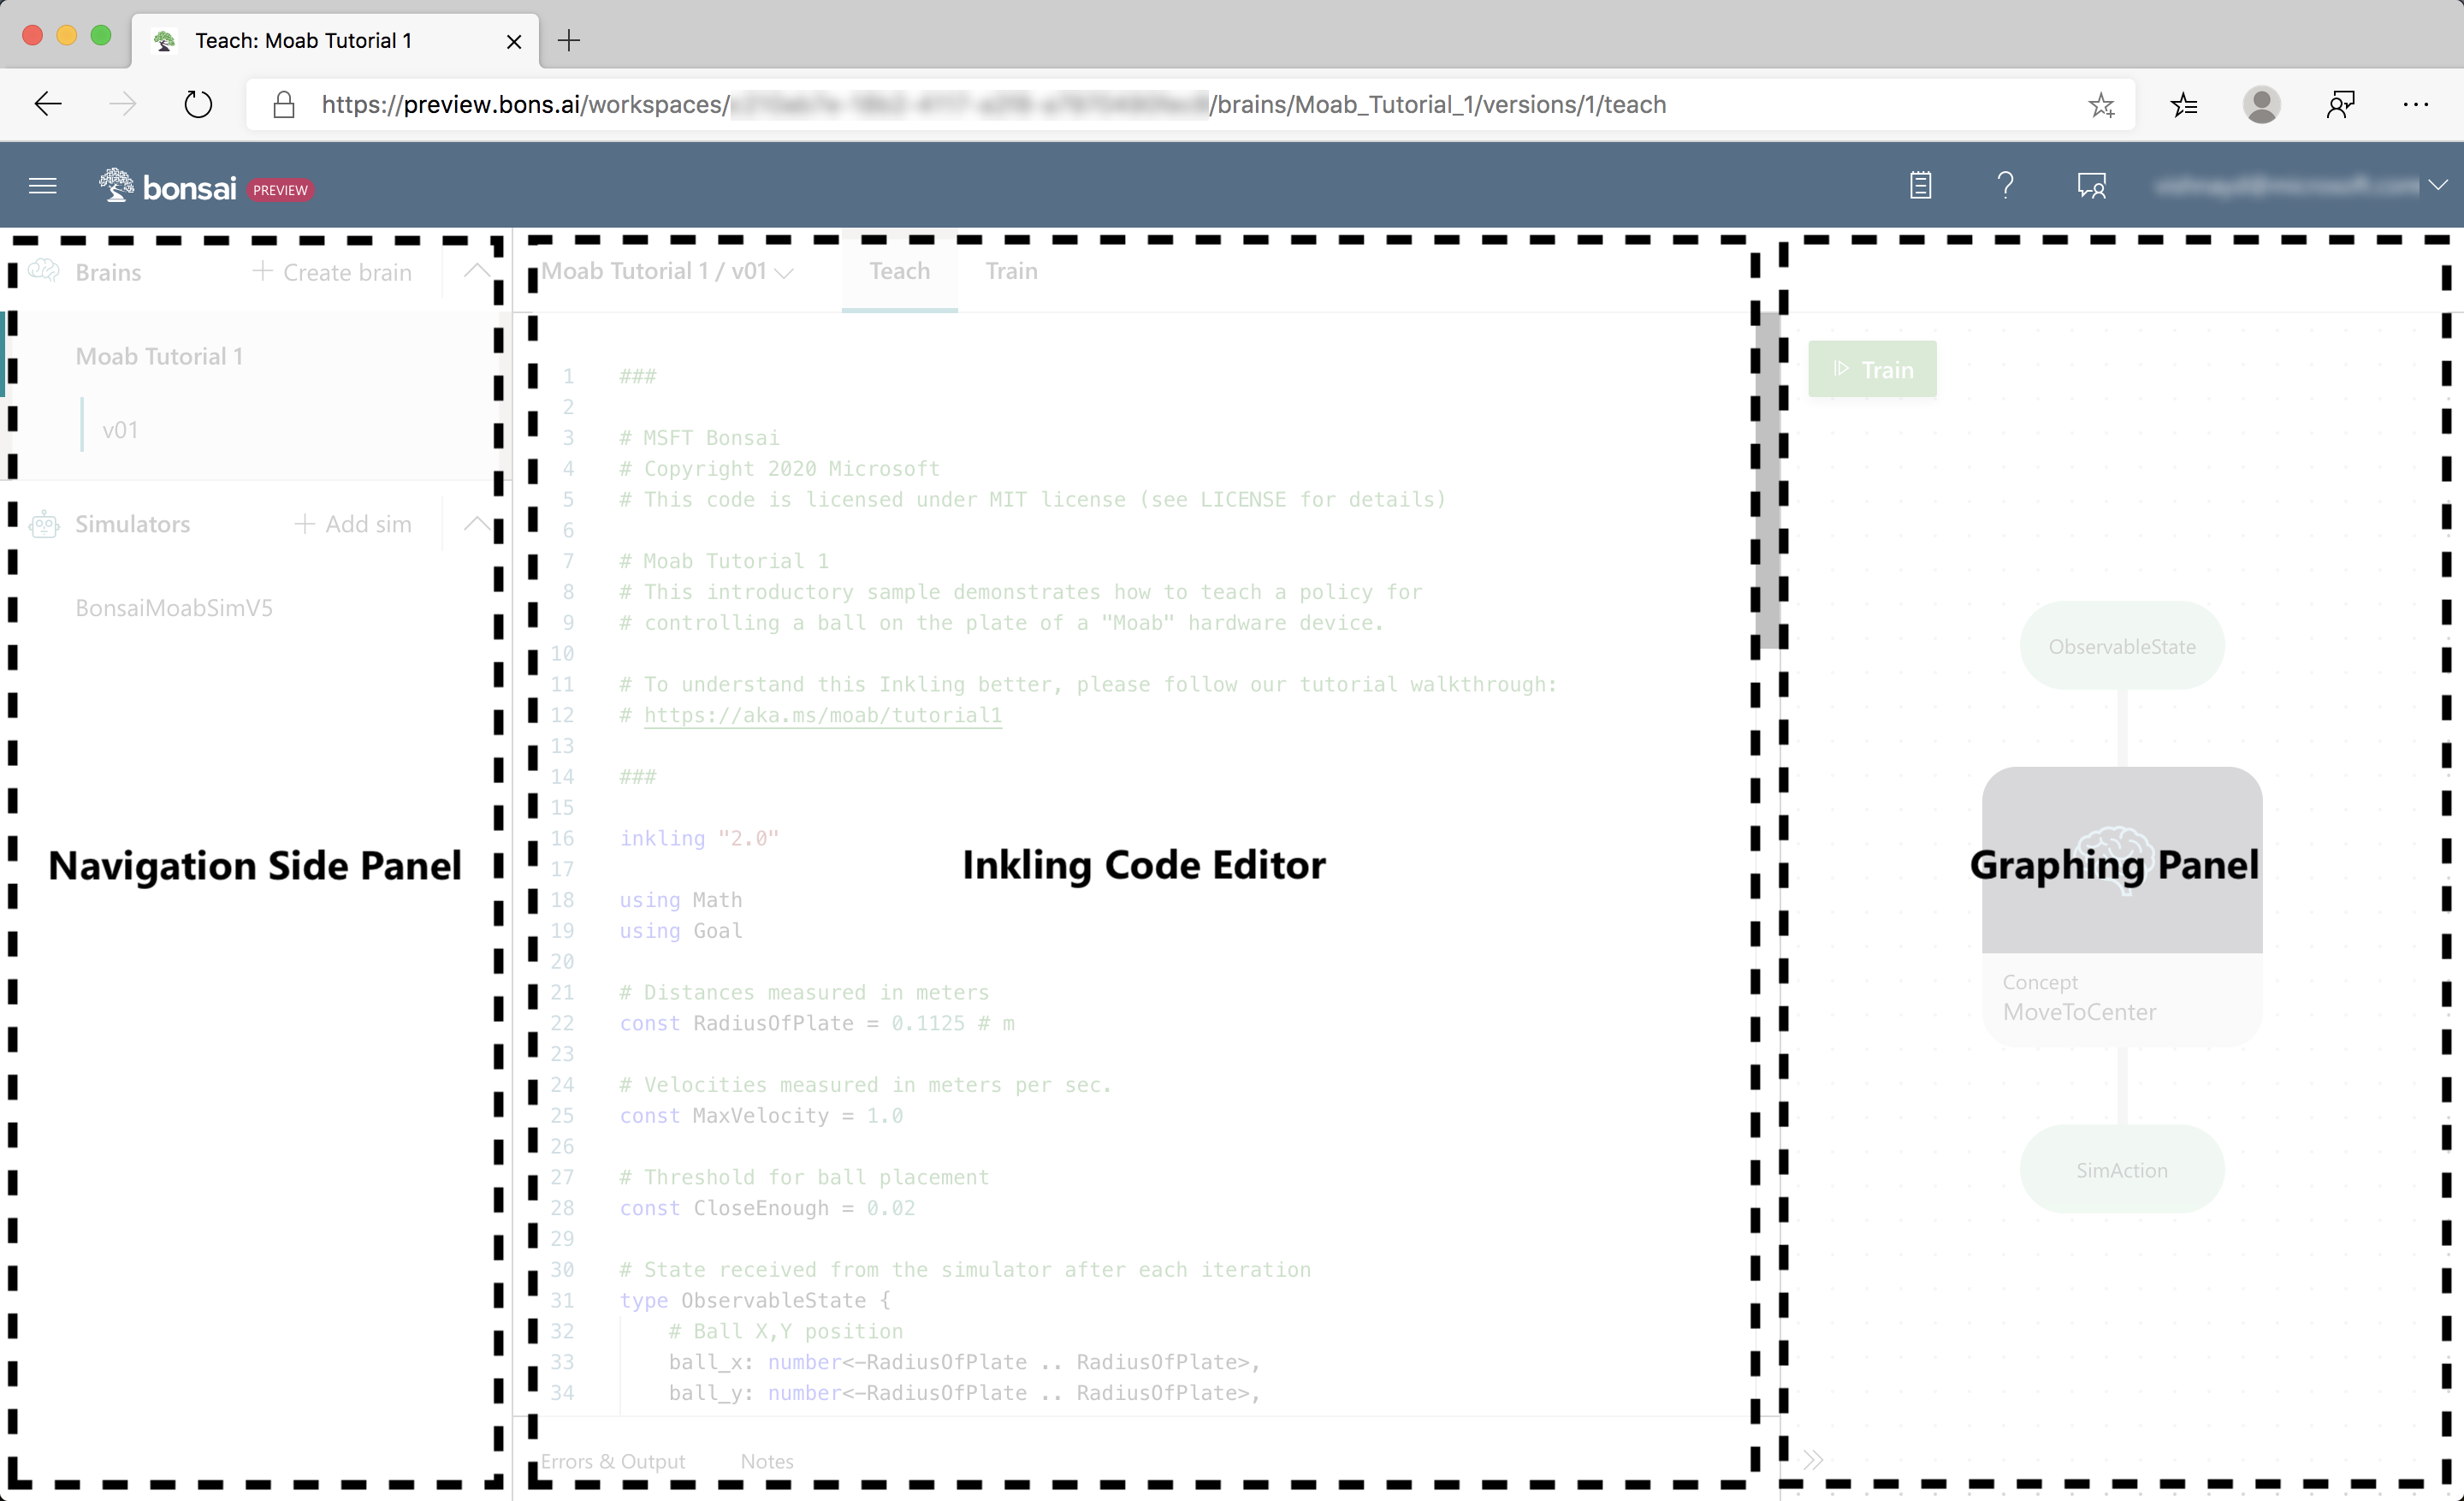
\includegraphics[width=1\textwidth]{Immagini/UI.png}}   
    \caption{Interfaccia di Bonsai}
    \label{fig:window}
\end{figure}

\subsubsection{Esecuzione del Modello}
A questo punto per eseguire il modello si può scegliere di farlo con un animazione: click destro su \texttt{AnimatedExperiment}, poi \texttt{Run} e dopo si visualizzerà in console la riuscita della registrazione alla piattaforma Bonsai tornare nella schermata dove è stato creato il brain. 
A questo punto si fa partire l'effettivo \texttt{train} del modello (azione diretta nel caso si sia scelto di eseguire un esperimento non animato), si vedrà quindi comparire un simulatore con il nome corrispondente su cui bisognerà cliccare.
\\ Nel caso fosse la prima volta che il brain viene eseguito potrebbero essere necessari diversi minuti per generare i parametri adatti e connettersi al simulatore. Si può far addestrare il brain per un lasso di tempo variabile, ma viene consigliato di tenere le iterazioni sotto le 1000, quando si ritiene siano sufficienti si cliccherà su \texttt{Stop Training}.

\subsubsection{Esportare e scalare il modello di Anylogic}
Il modello creato in AnyLogic necessita di essere esportato e compresso (\texttt{.zip}) per poter essere caricato su Bonsai. \\ Nel caso in cui si utilizzi \textit{AnyLogic Professional} sarà sufficiente selezionare nella barra dei menù \texttt{File > Export...> standalone Java application}, se si incontrassero delle difficoltà è disponibile il \href{https://anylogic.help}{supporto di Anylogic}.

Dopo questo passaggio è necessario importare il modello di Anylogic all'interno di Bonsai e per farlo sarà sufficiente selezionare su \texttt{Add sim} sull'interfaccia di Bonsai.
Si aprirà quindi la finestra di dialogo in figura \ref{fig:dialog} dove sarà sufficiente cliccare su AnyLogic, caricare il file \texttt{.zip} precedentemente creato e selezionare \texttt{Create simulator}. Il simulatore appena creato verrà visualizzato nella sezione \texttt{Simulators}.

\begin{figure}[!h]
    \centering
    \makebox[\textwidth][c]{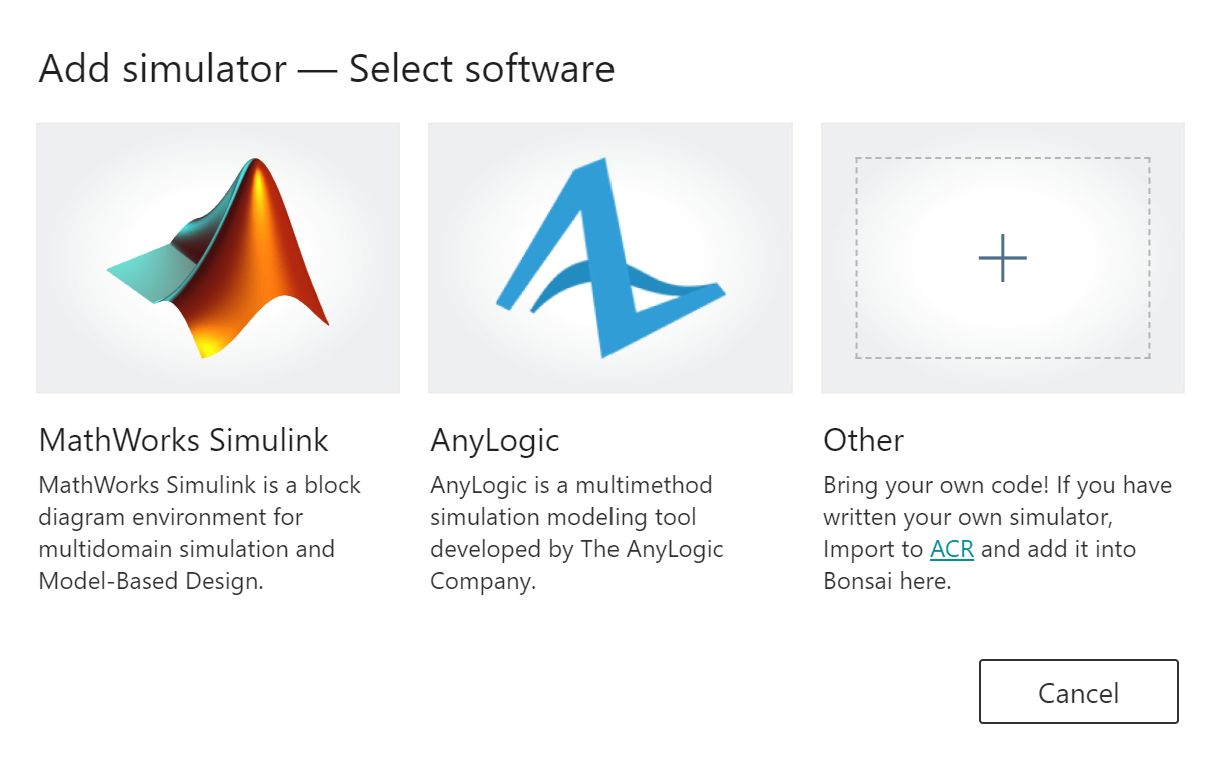
\includegraphics[width=1\textwidth]{Immagini/add_sim.png}}   
    \caption{Finestra per la scelta del simulatore}
    \label{fig:dialog}
\end{figure}
\clearpage
All'interno della scheda \texttt{Teach}, nella definizione del modello, è necessario aggiungere le seguenti linee di codice:

\begin{figure}[!h]
    \centering
    \makebox[\textwidth][c]{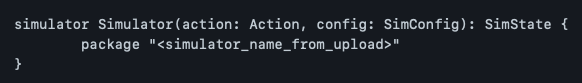
\includegraphics[width=1\textwidth]{Immagini/code.png}}   
    \label{fig:dialog}
\end{figure}

Si potrà quindi selezionare \texttt{Train} e dopo alcuni minuti si potranno vedere diversi simulatori collegati che addestrano il Brain. 

%----------------------------------------------------------------------

\subsection{H20.ai}
AnyLogic è partner di H2O.ai, una delle principali piattaforme di automatic machine learning. 
L’AutoML è una branca del ML che permette di applicare le tecniche di Ml ai problemi del mondo reale usando l’automazione. In particolare, automatizza la selezione, la composizione e la parametrizzazione dei modelli di machine learning.
L'obiettivo di integrare questi due sistemi è fornire la possibilità ai data scientist di testare le loro soluzioni in uno spazio sicuro e ai modellatori di accedere a una maggior quantità di input data-driven.

Le informazione per come utilizzare questa piattaforma con AnyLogic non sono accessibili al pubblico ma solo mettendosi in contatto con l'azienda. 
Le indicazioni che si possono ricavare dal \href{https://www.anylogic.com/features/artificial-intelligence/h2o-ai/}{sito di Anylogic} è la possibilità di scaricare da \textit{H2O.ai }il modello già addestrato per inserirlo all'interno delle simulazioni di AnyLogic ed utilizzarlo come fosse una funzione in grado di restituire delle predizioni basate sugl'input che vengono passati dinamicamente alla simulazione durante l'esecuzione.

%----------------------------------------------------------------------
\clearpage
\subsection{Pathmind}
La terza possibilità per inserire degli elementi di AI in AnyLogic è \textit{Pathmind}.
\\ Pathmind è una piattaforma SaaS che permette di avere accesso a delle tecniche di deep reinforcement learning e cloud computation per applicarle a degli scenari del mondo reale senza la necessità di avere esperienza di data science.

Pathmind a differenza dei servizi precedentemente presentati si va ad inserire all'interno di AnyLogic con Pathmind Helper attraverso cui è possibile agire sul modello.

Il processo da seguire per utilizzare Pathmind è il seguente: \begin{enumerate}
\item Creare un modello in AnyLogic che simuli un problema del mondo reale.
\item Usare Pathmind Helper per aggiungere il reinforcement learning all'interno della simulazione di AnyLogic.
\item Caricare la simulazione di AnyLogic in Pathmind, nel cui cloud avviene l'addestramento.
\item Scaricare i risultati ottenuti e validarli in AnyLogic.
\end{enumerate}

E' possibile trovare informazioni aggiuntive su Pathmind nel \href{https://help.pathmind.com/en/collections/2106204-tutorials-example-simulation-models#getting-started}{help} mantenuto dall'azienda. 

\clearpage
\subsubsection{Pathmind Helper}
All'interno di ogni agente che vogliamo dotare di AI abbiamo bisogno di creare un diagramma di stato e inserire Pathmind Helper come nell'esempio in figura \ref{fig:AIagent}. 

\begin{figure}[!h]
    \centering
    \makebox[\textwidth][c]{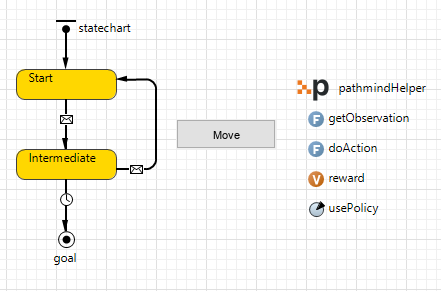
\includegraphics[width=200px]{Immagini/aiagent.png}}   
    \caption{Agente tipo}
    \label{fig:AIagent}
\end{figure}

Aprendo Pathmind Helper possiamo controllare i seguenti elementi del RL:
\begin{itemize}
\item \textbf{Number of Agents}: il numero di agenti "controllati" presenti nel modello.
\item \textbf{Observations}: contengono tutte le informazioni sullo stato corrente dell'ambiente.
\item \textbf{Metrics}: sono le metriche che vengono utilizzate all'interno della funzione di \textit{reward} per determinare se un'azione è stata buona o cattiva, a volte contiene anche il costo di essa. 
\item \textbf{Actions}: definisce tutte le azioni che un agente può svolgere.
\item \textbf{Done}: dal momento che tutte le simulazioni hanno necessità di un punto di arrivo, questo viene settato o dopo un lasso di tempo prestabilito o al raggiungimento di una determinata condizione.
\item \textbf{Event Trigger}: indicano a Pathmind quando inizia l'azione successiva, dopo un lasso di tempo o al verificarsi di una determinata condizione. 
\end{itemize}




All'interno di Pathmind Helper è possibile testare il modello, prima di esportarlo, spuntando la \texttt{Debug Mode} che permetterà di aprire il \texttt{Developer Panel} al cui interno, 
in caso in cui fosse tutto impostato correttamente, verrà stampata a video ogni azione che l'agente performa (figura \ref{fig:debugfig}).

\begin{figure}[!h]
    \centering
    \makebox[\textwidth][c]{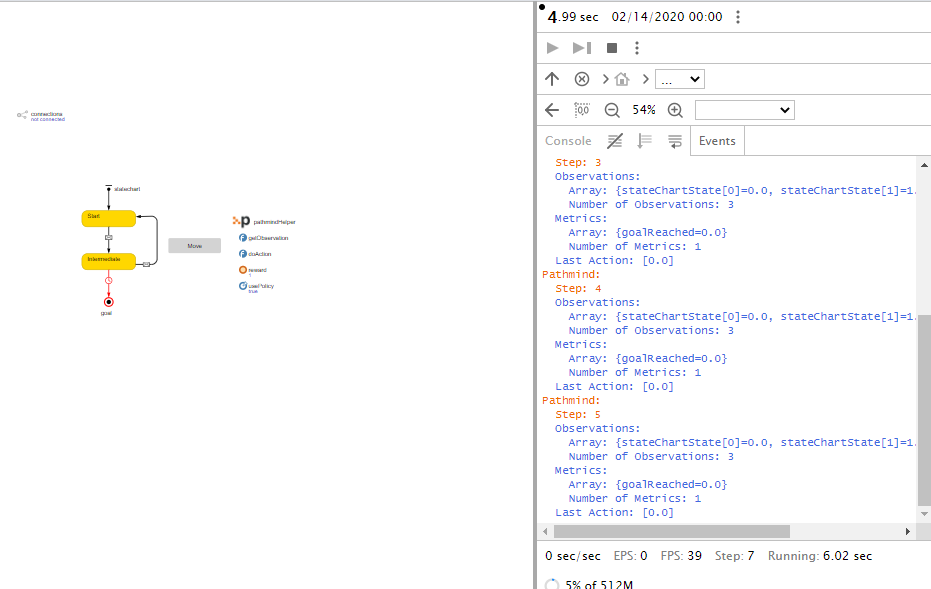
\includegraphics[width=1\textwidth]{Immagini/debug.png}}   
    \caption{Agente tipo}
    \label{fig:debugfig}
\end{figure}

Dopo che il modello è stato configurato è possibile esportarlo nell'applicazione web di Pathmind per l'addestramento. All'interno di questa web app è possibile configurare la funzione di reward ed addestrare con essa il modello in circa 10 minuti. 

Al termine dell'addestramento è possibile esportare la policy risultante e inserirla in Anylogic all'interno del Pathmind helper sotto \texttt{Policy File}. Seguendo la policy inserita l'agente convergerà all'obbiettivo nel minor numero di passi possibile.







